% bab3.tex - Rancangan dan Implementasi Aplikasi (proposal Bab III ditulis ulang sesuai yang dibangun).
% Sumber: src/cli/landcover.cpp, app/landcover/{contract,labeling,export}.py, app/tools/README.md,
% web/README.md, web/package.json, app/requirements.txt, Makefile. TANPA angka kinerja (ada di Bab V).
\chapter{RANCANGAN DAN IMPLEMENTASI APLIKASI}

\section{Gambaran Umum}
Pengguna, yaitu analis lingkungan atau perencana wilayah, memilih atau mengunggah citra suatu wilayah, lalu memilih jumlah kelompok $K$, jumlah iterasi, dan mode eksekusi. Aplikasi menyediakan dua mode:
\begin{itemize}
    \item \textbf{Mode CPU saja (L0)}: seluruh tahap berjalan serial di CPU. Mode ini menjadi \emph{baseline}.
    \item \textbf{Mode Optimalisasi}: setiap tahap berjalan pada perangkat terbaiknya. K-Means dijalankan dengan OpenMP atau CUDA yang dipilih otomatis berdasarkan besar pekerjaan (Subbab~\ref{sec:otomatis}), sedangkan tahap pendukung memakai OpenMP.
\end{itemize}

Antarmuka berupa aplikasi web dengan dua halaman. Halaman \textbf{Pemetaan} melayani alur kerja analis: memilih citra dan $K$, menekan ``Buat peta'' (mode Optimalisasi), membandingkan citra asli dengan peta kelas, memberi nama setiap kelompok, membaca tabel persentase dan luas, lalu mengekspor hasilnya. Halaman \textbf{Kinerja} melayani pembuktian optimasi: menjalankan mode CPU saja dan mode Optimalisasi pada citra dan parameter yang sama, lalu menampilkan waktu total, \emph{speedup}, grafik waktu per tahap beserta perangkat yang mengerjakannya, dan status verifikasi hasil antarmode.

\section{Arsitektur dan Alur Proses}
\label{sec:arsitektur}
Aplikasi terdiri dari dua bagian yang dihubungkan oleh kontrak berkas. Bagian pertama berjalan di Windows: antarmuka web (React) dan API (FastAPI, \kode{app/api}) yang memakai logika murni di \kode{app/services} dan \kode{app/landcover}. Bagian kedua adalah program inti \kode{landcover} (C++, \kode{src/cli/landcover.cpp}) yang dibangun dan dijalankan di WSL 2. API memanggil \kode{landcover} lewat \kode{CliLauncher} (\kode{app/launchers/cli.py}) dan pembungkus \kode{app/tools/lc\_wsl.cmd}, yang mengubah \emph{path} Windows menjadi \emph{path} WSL lalu menjalankan program di dalam WSL. Program inti menulis hasilnya ke sebuah folder \emph{run}; API membaca folder itu melalui \kode{app/landcover/contract.py} dan mengirim ringkasan ke antarmuka. Antarmuka tidak pernah memuat citra atau label resolusi penuh.

Di dalam \kode{landcover}, citra melewati enam tahap berurutan. Citra Sentinel-2 dalam format GeoTIFF atau JPEG2000 dikonversi lebih dulu menjadi PNG dengan GDAL (\kode{gdal\_translate}) dan dipotong menjadi ukuran 512, 1024, dan 2048 piksel; konversi ini adalah tahap persiapan data dan tidak termasuk waktu yang diukur. Alur lengkap beserta perangkat setiap tahap pada mode Optimalisasi ditunjukkan pada Gambar~\ref{fig:arsitektur}.

\begin{figure}[H]
\centering
\begin{tikzpicture}[
    simpul/.style={draw=black!70, fill=simpulserial, rounded corners=2pt, align=center, minimum height=1.25cm, text width=1.95cm, font=\small, inner sep=2pt},
    lapis/.style={simpul, fill=white, text width=2.2cm},
    panah/.style={-{Stealth}, thick},
    ket/.style={font=\scriptsize, align=center}]
% Baris atas: lapisan aplikasi (Windows)
\node[lapis] (ui)  at (0,0)     {UI web\\ (React)};
\node[lapis] (api) at (3.4,0)   {API\\ (FastAPI)};
\node[lapis] (cli) at (6.8,0)   {{\ttfamily\footnotesize CliLauncher}\\ + {\ttfamily\footnotesize lc\_wsl}};
\node[lapis] (run) at (12.75,0) {Folder \emph{run}\\ (JSON, PNG,\\ \kode{labels.u8})};
% Baris tengah: tahap di dalam landcover (WSL)
\node[simpul] (baca)  at (0,-3)     {Baca PNG\\ (\emph{serial})};
\node[simpul] (init)  at (2.55,-3)  {Inisialisasi \emph{centroid}\\ (\emph{serial})};
\node[simpul, fill=simpulcuda] (km) at (5.1,-3) {K-Means\\ (CUDA /\\ OpenMP)};
\node[simpul, fill=simpulomp] (cnt) at (7.65,-3) {\emph{Counts} dan \emph{nodata}\\ (OpenMP)};
\node[simpul, fill=simpulomp] (warna) at (10.2,-3) {Pewarnaan peta\\ (OpenMP)};
\node[simpul, fill=simpulomp] (tulis) at (12.75,-3) {Tulis PNG\\ (OpenMP per \emph{strip})};
\node[simpul, fill=simpulcuda] (iter) at (5.1,-5) {\emph{Assignment} + \emph{update} $\times$ iterasi tetap};
% Kotak program landcover
\begin{scope}[on background layer]
\node[draw=black!50, dashed, rounded corners=3pt, inner sep=6pt, fit=(baca) (tulis) (iter)] (box) {};
\end{scope}
\node[ket, anchor=south west] at (box.north west) {program \texttt{landcover} (C++, WSL)};
% Panah
\draw[{Stealth}-{Stealth}, thick] (ui) -- node[ket, above] {HTTP} (api);
\draw[panah] (api) -- (cli);
\draw[panah] (cli.south) -- (cli.south |- box.north);
\draw[panah] (baca) -- (init);
\draw[panah] (init) -- (km);
\draw[panah] (km) -- (cnt);
\draw[panah] (cnt) -- (warna);
\draw[panah] (warna) -- (tulis);
\draw[panah] ([xshift=-4pt]km.south) -- ([xshift=-4pt]iter.north);
\draw[panah] ([xshift=4pt]iter.north) -- ([xshift=4pt]km.south);
\draw[panah] (tulis.north |- box.north) -- (run.south);
\draw[panah] (run.north) to[out=160, in=20] node[ket, above] {dibaca \texttt{contract.py}} (api.north);
\end{tikzpicture}
\caption{Arsitektur aplikasi dan alur proses mode Optimalisasi. Warna simpul menunjukkan perangkat: abu-abu = CPU serial, hijau = OpenMP, jingga = CUDA atau OpenMP (dipilih otomatis). Pada mode CPU saja semua tahap \kode{landcover} berjalan serial}
\label{fig:arsitektur}
\end{figure}

\section{Kontrak Data}
\label{sec:kontrak}
Antarmuka dan program inti hanya berbagi dua hal: opsi baris perintah \kode{landcover} dan isi folder \emph{run}. Dengan kontrak ini, implementasi tiruan (\kode{MockLauncher}) dan program inti asli dapat dipertukarkan tanpa mengubah antarmuka. Opsi utama ditunjukkan pada Tabel~\ref{tab:opsi}.

\begin{table}[H]
\centering
\caption{Opsi utama program \kode{landcover}}
\label{tab:opsi}
\begin{tabularx}{\textwidth}{|L{4.3cm}|Y|}
\hline
\hdr{Opsi} & \hdr{Arti} \\ \hline
\kode{-{}-mode cpu|opt} & Mode CPU saja (L0) atau mode Optimalisasi \\ \hline
\kode{-{}-kmeans auto|omp|cuda} & Implementasi K-Means pada mode Optimalisasi; bawaan \kode{auto} (Subbab~\ref{sec:otomatis}) \\ \hline
\kode{-{}-input} & Satu berkas PNG, atau folder berisi potongan PNG dan \kode{manifest.json} \\ \hline
\kode{-{}-k}, \kode{-{}-iters}, \kode{-{}-seed} & Jumlah kelompok (1--16), jumlah iterasi tetap, dan \emph{seed} inisialisasi \\ \hline
\kode{-{}-threads} & Jumlah \emph{thread} OpenMP pada mode Optimalisasi \\ \hline
\kode{-{}-out} & Folder \emph{run} tujuan \\ \hline
\kode{-{}-write-labels} & Menulis label resolusi penuh (\kode{labels.u8}) untuk verifikasi dan ekspor \\ \hline
\kode{-{}-info} & Mencetak kemampuan \emph{build} (mesin K-Means yang terhubung dan ambang otomatis) dalam JSON \\ \hline
\end{tabularx}
\end{table}

Isi folder \emph{run} ditunjukkan pada Tabel~\ref{tab:folderrun}. Setiap berkas ditulis ke berkas sementara lalu diganti nama, dan \kode{meta.json} ditulis paling akhir sebagai tanda bahwa \emph{run} lengkap. \emph{Run} yang gagal di tengah tidak pernah tampak valid bagi antarmuka.

\begin{table}[H]
\centering
\caption{Isi folder \emph{run}}
\label{tab:folderrun}
\begin{tabularx}{\textwidth}{|L{4.3cm}|Y|}
\hline
\hdr{Berkas} & \hdr{Isi} \\ \hline
\kode{meta.json} & Parameter, mode, mesin K-Means yang dipakai beserta alasan pemilihan otomatis, ukuran citra, statistik \emph{nodata}, dan informasi pemanasan CUDA \\ \hline
\kode{timing.json} & Waktu per tahap dalam milidetik (kunci berakhiran \kode{\_ms}) dan perangkat setiap tahap \\ \hline
\kode{centroids.json} & $K$ \emph{centroid} akhir (R, G, B) \\ \hline
\kode{counts.json} & Jumlah piksel per kelompok dari label resolusi penuh \\ \hline
\kode{labels\_preview.png}, \kode{map\_preview.png} & Pratinjau label dan peta beresolusi kecil untuk antarmuka \\ \hline
\kode{map.png} & Peta kelas resolusi penuh \\ \hline
\kode{labels.u8} & Label resolusi penuh, satu \emph{byte} per piksel (opsional, \kode{-{}-write-labels}) \\ \hline
\kode{verification.json} & Hasil modul verifikasi antarmode (opsional; tidak ditulis oleh \kode{landcover}) \\ \hline
\end{tabularx}
\end{table}

Pembagian waktu di \kode{timing.json} sama untuk kedua mode. Waktu baca, pewarnaan, dan tulis diukur oleh \kode{landcover}, sedangkan waktu inisialisasi dan K-Means diisi oleh fungsi \kode{kmeans\_*} (pada CUDA ditambah rincian salin ke GPU, \emph{kernel}, dan salin kembali). Waktu total adalah jumlah waktu baca, waktu dinding pemanggilan K-Means, pewarnaan, dan tulis. Dua kelompok pekerjaan sengaja tidak dimasukkan ke waktu total, tetapi tetap dicatat terpisah:
\begin{itemize}
    \item \textbf{Pekerjaan pendamping} (\kode{aux\_ms}): menghitung \emph{counts} dan \emph{nodata}, membuat pratinjau, dan menulis \kode{labels.u8}. Pekerjaan ini hanya melayani antarmuka, sehingga opsi \kode{-{}-write-labels} tidak mengubah angka \emph{benchmark}.
    \item \textbf{Pemanasan CUDA} (\kode{warmup\_ms}): sebelum K-Means diukur, \kode{landcover} memanggil \kode{kmeans\_cuda} sekali pada citra $64\times64$ agar inisialisasi konteks CUDA tidak tercampur ke waktu K-Means. Biaya ini tetap dirasakan pengguna pada setiap proses baru, sehingga Bab~V menyajikan juga waktu proses keseluruhan.
\end{itemize}

\section{Antarmuka}
\label{sec:antarmuka}
Halaman Pemetaan ditunjukkan pada Gambar~\ref{fig:uipemetaan} dan Gambar~\ref{fig:uiluas}, dan halaman Kinerja pada Gambar~\ref{fig:uikinerja}. Semua tangkapan layar diambil dengan citra Sentinel-2 asli berukuran $2048\times2048$ piksel, $K=8$, dan program \kode{landcover} asli (bukan data tiruan). Pratinjau di layar berukuran paling besar $1024$ piksel, sedangkan persentase dan luas dihitung dari \emph{counts} seluruh piksel.

\begin{figure}[H]
\centering
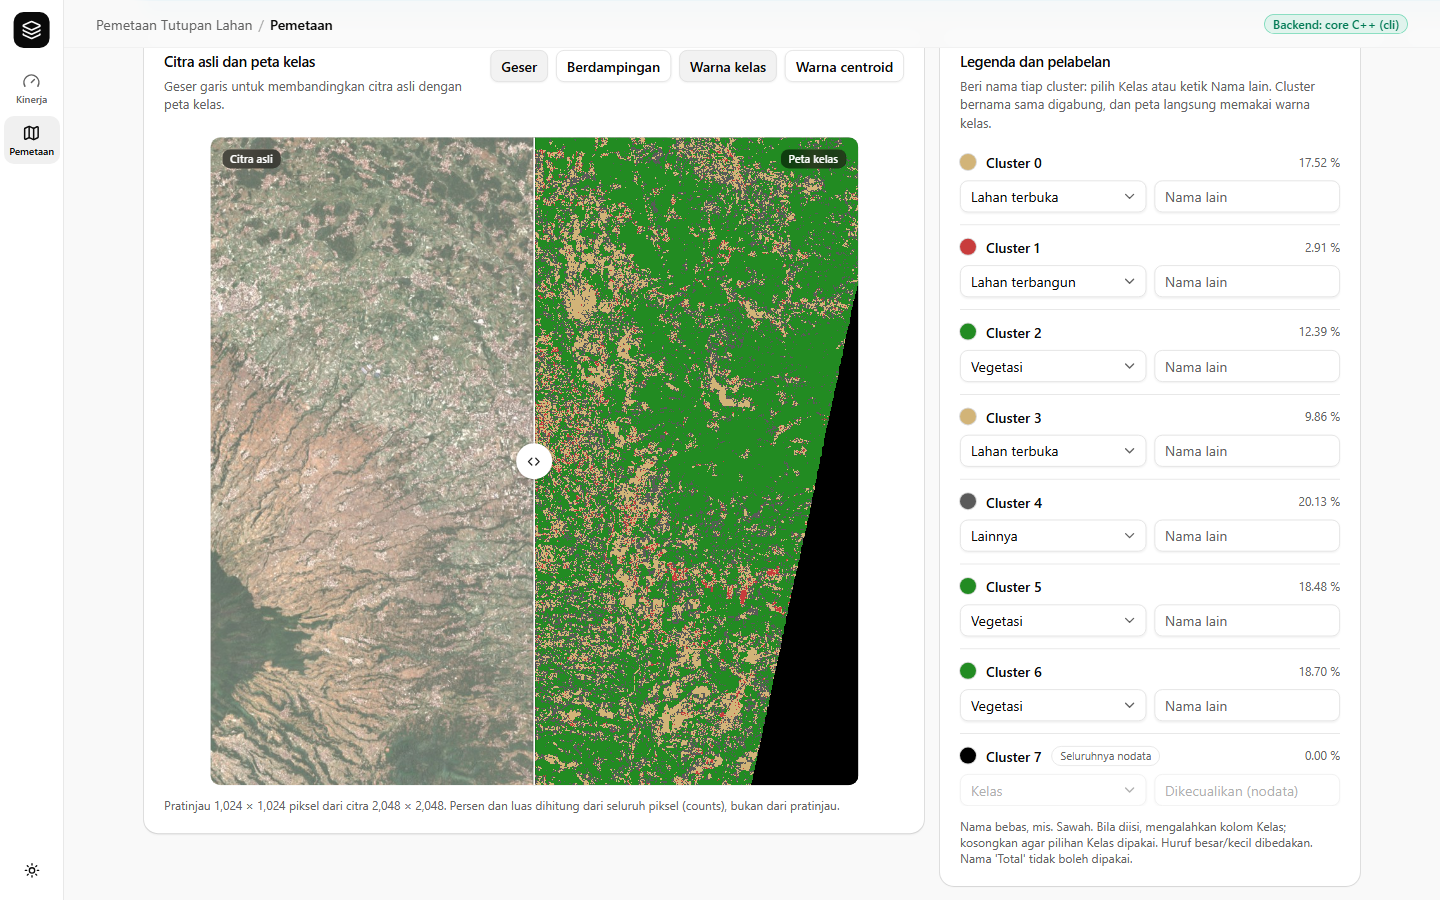
\includegraphics[width=0.95\textwidth]{ui_pemetaan_citra_vs_peta.png}
\caption{Halaman Pemetaan: citra asli dan peta kelas dengan penggeser sebelum/sesudah, serta legenda yang sekaligus menjadi panel pelabelan}
\label{fig:uipemetaan}
\end{figure}

\begin{figure}[H]
\centering
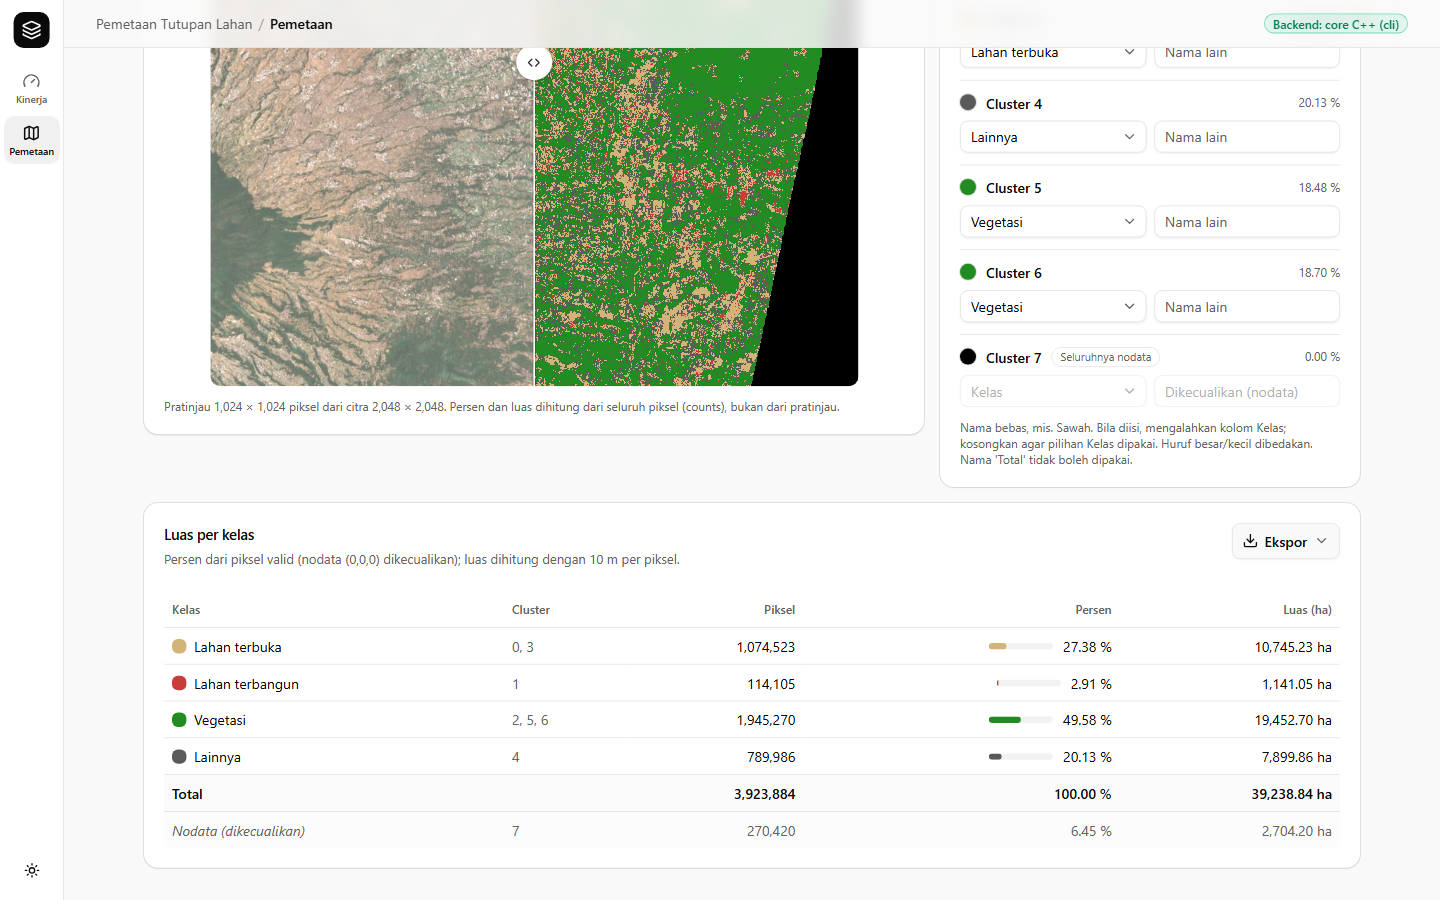
\includegraphics[width=0.95\textwidth]{ui_pemetaan_legenda_luas.png}
\caption{Halaman Pemetaan: tabel persentase dan luas per kelas, dengan baris \emph{nodata} yang dikecualikan dan menu ekspor}
\label{fig:uiluas}
\end{figure}

\begin{figure}[H]
\centering
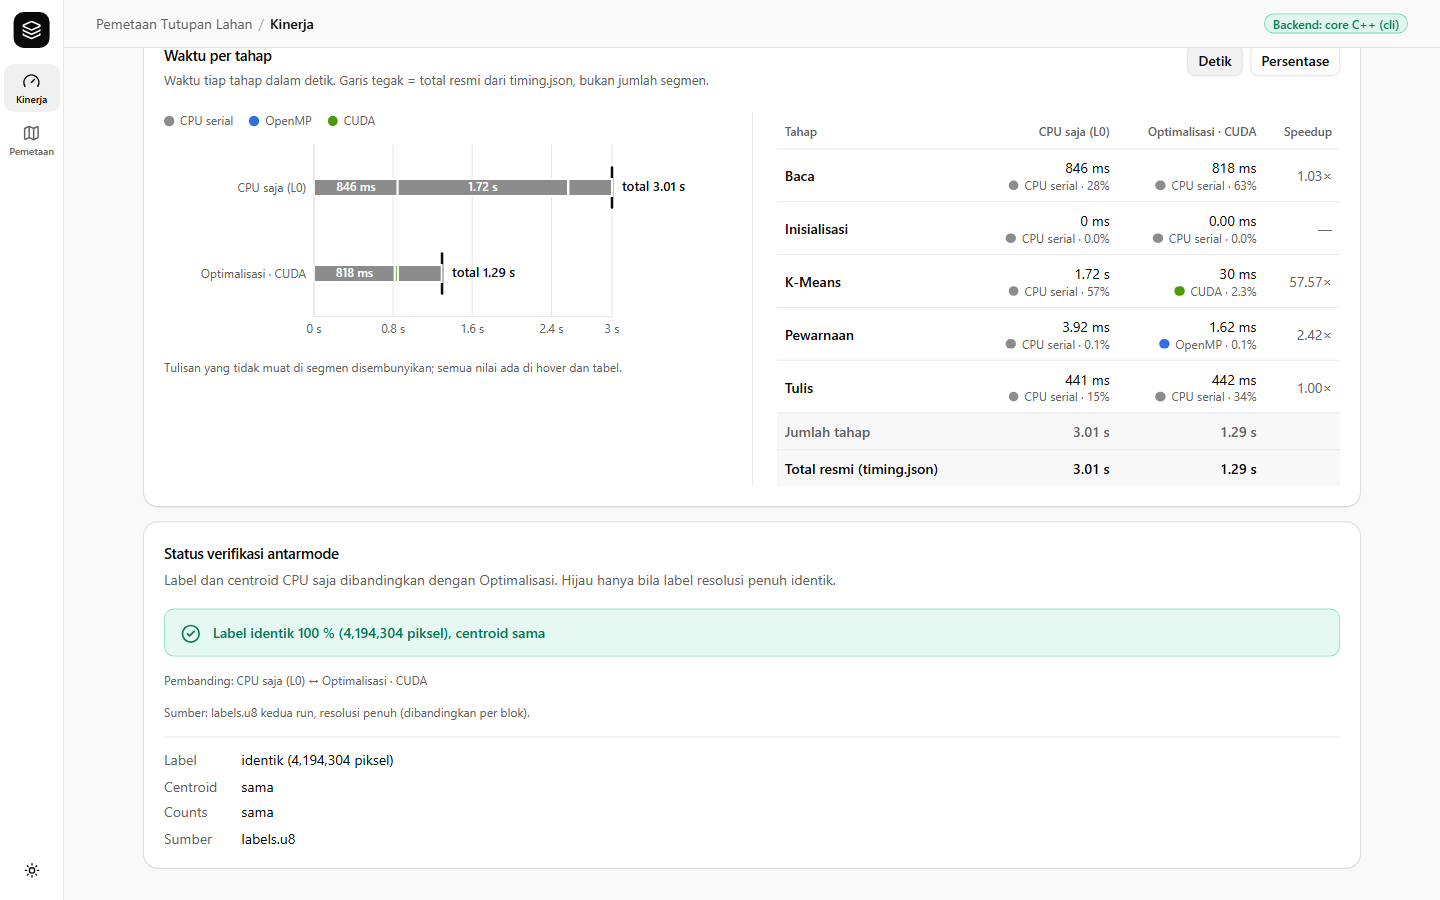
\includegraphics[width=0.95\textwidth]{ui_kinerja_tahap_verifikasi.png}
\caption[Halaman Kinerja: waktu per tahap beserta perangkatnya dan status verifikasi antarmode]{Halaman Kinerja: waktu per tahap beserta perangkatnya dan status verifikasi antarmode. Tangkapan layar ini hanya menunjukkan tata letak; angka di dalamnya berasal dari laptop uji fungsional dengan \emph{build} lama dan bukan hasil kinerja resmi (Bab~V). Pada \emph{build} itu \kode{kmeans\_omp} belum terhubung ke \kode{landcover}; pada \kode{main} OpenMP sudah terhubung dan mode otomatis memakai ambang $N\times K$}
\label{fig:uikinerja}
\end{figure}

\section{Pelabelan dan Perhitungan Luas}
\label{sec:pelabelan}
Setiap kelompok diberi nama kelas dari daftar pilihan (vegetasi, air, lahan terbangun, lahan terbuka, awan/bayangan, lainnya) atau nama bebas. Beberapa kelompok boleh diberi nama yang sama sehingga tergabung menjadi satu kelas, dan peta langsung diwarnai ulang menurut kelasnya. Nama kelas per \emph{run} disimpan di peramban dan dikirim ke API saat tabel luas diminta.

Semua angka luas berasal dari \kode{counts.json}, yaitu jumlah piksel bilangan bulat per kelompok dari label resolusi penuh, bukan dari pratinjau (\kode{app/landcover/labeling.py}). Piksel \emph{nodata} $(0,0,0)$ selalu jatuh ke satu kelompok yang sama; \kode{landcover} memeriksa hal ini, dan jumlahnya dikurangkan dari kelompok tersebut. Untuk kelas $k$ yang terdiri atas himpunan kelompok $C_k$, dengan $n_j$ jumlah piksel kelompok $j$, $N$ jumlah piksel citra, $N_{\text{nodata}}$ jumlah piksel \emph{nodata}, dan $s$ ukuran piksel dalam meter,
\begin{equation}
    \text{persen}_k = \frac{100 \sum_{j \in C_k} n'_j}{N - N_{\text{nodata}}}, \qquad
    \text{luas}_k = \frac{s^2 \sum_{j \in C_k} n'_j}{10\,000}\ \text{ha},
    \label{eq:luas}
\end{equation}
dengan $n'_j$ jumlah piksel kelompok $j$ setelah piksel \emph{nodata} dikurangkan. Untuk resolusi 10 meter, satu piksel sama dengan 0,01~ha. Kelompok berjumlah nol piksel sah (misalnya bila $K$ lebih besar daripada jumlah warna unik) dan ditampilkan sebagai 0\%, tanpa pembagian dengan jumlah piksel kelompok. Hasil dapat diekspor sebagai PNG pratinjau, CSV luas per kelas, CSV per kelompok, dan PNG peta resolusi penuh yang dibuat dari \kode{labels.u8} (\kode{app/landcover/export.py}).

\section{Stack Teknologi}
\label{sec:stack}
\emph{Stack} teknologi yang dipakai ditunjukkan pada Tabel~\ref{tab:stack}. Dibandingkan usulan di proposal, ada tiga perubahan: antarmuka memakai web React dengan API FastAPI (Streamlit hanya tersisa sebagai cadangan), \emph{build} memakai Make (bukan CMake), dan penulisan PNG memakai penulis paralel buatan sendiri.

\begin{table}[H]
\centering
\caption{\emph{Stack} teknologi yang dipakai}
\label{tab:stack}
\begin{tabularx}{\textwidth}{|L{4cm}|Y|}
\hline
\hdr{Komponen} & \hdr{Pilihan} \\ \hline
Inti pemrosesan & C++17 dan OpenMP (GCC 13.3), CUDA C++ (\kode{nvcc} 12.9, \kode{-arch=sm\_86}), semuanya dengan \kode{-O3} \\ \hline
Baca/tulis citra & Baca dengan \kode{stb\_image}; tulis dengan penulis PNG paralel sendiri (\kode{src/cli/png\_io\_omp.cpp}, bawaan Makefile), \kode{stb\_image\_write} tetap tersedia sebagai cadangan \\ \hline
Persiapan data & GDAL (\kode{gdal\_translate}) untuk konversi dan pemotongan kanal Sentinel-2 menjadi PNG \\ \hline
Pengukuran & \emph{Timer} per tahap di dalam program dan CUDA \emph{events} \\ \hline
\emph{Build} & GNU Make di Linux (WSL 2) \\ \hline
Antarmuka & React, TypeScript, Vite, Tailwind CSS, shadcn/ui, Recharts, dan TanStack Query, dengan API FastAPI dan uvicorn (Python) \\ \hline
Analisis data & Python (skrip di \kode{bench/}) untuk tabel dan grafik \\ \hline
Pengujian & \kode{pytest} untuk aplikasi; program uji C++ untuk inti \\ \hline
\end{tabularx}
\end{table}

\section{Pengujian Perangkat Lunak}
\label{sec:pengujianpl}
Pengujian dilakukan di dua lapis.
\begin{itemize}
    \item \textbf{Inti (C++, WSL):} \kode{test\_ref} menguji referensi CPU; \kode{test\_cuda\_vs\_ref} membandingkan setiap varian CUDA dengan referensi pada banyak ukuran citra dan nilai $K$; \kode{test\_omp\_vs\_cpu} membandingkan \kode{kmeans\_omp} dengan \kode{kmeans\_cpu}; \kode{test\_png\_omp} memastikan PNG dari penulis paralel terdekode menjadi piksel yang sama persis dengan masukan untuk berbagai jumlah \emph{thread}. Semua dijalankan lewat target Make (\kode{make test}, \kode{make test-omp}, \kode{make test-png-omp}).
    \item \textbf{Aplikasi (Python):} \kode{pytest} menguji pembaca kontrak, pelabelan dan luas, ekspor, API, peluncur, dan logika tampilan, termasuk tes dengan program \kode{landcover} asli lewat pembungkus WSL.
\end{itemize}
Hasil pengujian ini dirangkum di Subbab~\ref{sec:hasilverifikasi}.
